\documentclass[a4paper, 11 pt, conference]{article}
\usepackage{color}

\usepackage{hyperref}
\usepackage{graphicx}
\usepackage{url}


\title{\textbf{Productizing TLS Attacks:} \\
	 \textbf{The Rupture API}}

\author{
	Eva Sarafianou\footnotemark[1]\\
	National Techical University of Athens\\
	University of Athens\\
	eva.sarafianou@gmail.com\\
	\and
	Dionysis Zindros\footnotemark[1]\\
	University of Athens\\
	dionyziz@di.uoa.gr\\
	\and
	Aggelos Kiayias\thanks{Research supported by ERC project CODAMODA, project \#259152.}\\
	University of Edinburgh\\
	akiayias@inf.ed.ac.uk\\
	}
	
\date{}
\pagenumbering{arabic}

\begin{document}
	
\maketitle
	
\begin{abstract}
All the side-channel attacks against TLS are based on common premises: Hooking the browser, making a large number of specially crafted requests, collecting and analyzing network data. Although there are several frameworks for solely hooking the browser, such as BeEF, and special tools for capturing network data, such as bettercap, the strategy and analysis parts of the attack have not been previously automated. 
	
In this presentation, we extend Rupture, a generic browser TLS side-channel attack framework that was presented in Black Hat Asia 2016, with a new, open source, usable RESTful API and web interface. We take advantage of the modularity of Rupture to create a robust RESTful API. Our API uses the existing Rupture modules --- the client, injector, sniffer and backend consisting of the strategy and analyzer components --- which have high expressibility so that any side-channel TLS attack such as for example all of CRIME, BREACH, POODLE, TIME, HEIST or BEAST can be implemented.

We will show a demo of the RESTful API and web interface. We will configure a victim and launch a complete BREACH attack against a target in order to illustrate the automation and usability of the API and the web interface.
\end{abstract}
	
\section{Introduction}
	Rupture~\cite{c15} is a general side-channel attack framework. It can be used to conduct network attacks against TLS web services. It is focused on compression side-channel attacks~\cite{c17}, but provides a generalized scalable system for performing any attack on web services which requires a persistent command-and-control channel along with attack adaptation.
	
	Our contributions in this work are a RESTful API that enables researchers to
	fully automate TLS-based attacks such as compression side-channel attacks. We
	provide a usable, clean set of end-points which can be used to mount the
	attack: Managing targets such as various web services, managing victims by
	robustly injecting and sniffing for information on local networks based on IP
	addresses, managing strategies for advancing attack rounds based on state
	search exploration, and running analyses on collected data, which is stored
	persistently. We are confident this automation will enable cryptographers and
	security researchers to heavily experiment with the various attack parameters,
	yielding better attack results in terms of correctness and performance.
	
Our contribution also includes an easy to use web interface, based on our API, which allows readily mounting sophisticated TLS attacks such as compression side-channel attacks. 
	
	Many advanced attacks against TLS such as the AES extensions to BREACH have still not been mitigated. There is a widespread view in the industry that these attacks are impractical to mount even for resourceful adversaries, and, since they are difficult to mitigate, they have been ignored and put under the rug. However, we insist that these attacks are very practical to conduct for advanced adversaries. We have automated these attacks and significantly improved the usability of performing them in order to illustrate that any attacker can readily exploit such vulnerabilities. Providing an open-source implementation of this automation for the white hat community is actively helping understand how these attacks remain within the realm of practicality.
	
	Rupture was designed because all the available attack tools to conduct CRIME~\cite{c1}, BREACH~\cite{c3} and POODLE~\cite{c2} attacks before Rupture were at the proof-of-concept level and did not provide a productized robust system that that can easily be used in real conditions. In our previous work~\cite{c15}, we spent a lot of time building separate proof-of-concept implementations of BREACH and invested a lot of time to mount attacks against specific end-points. The biggest struggle was that it takes a lot of effort to conduct such an attack without the appropriate tools. 
	
	Rupture made it easier to mount such attacks and provide reasonable pre-configured defaults, targets, and attack strategies that can be used in practice or modified to suit the need of new attacks. The RESTful API and web interface for Rupture makes mounting such attacks completely automated. The framework is designed specifically to allow for further investigations on both the practical and theoretical side. On the practical side, our network sniffing and injection components are modular and replaceable. On the theoretical side, our analysis and strategy core is independent of data collection means, allowing researchers to verify or reject statistical analysis hypotheses through experimental adaptive sample collection.
	
	In our presentation, we will show a demo of our RESTful API and web interface for Rupture. We will configure a victim and initiate an attack to one of the possible targets to show both the automated way it is performed and also the clear and user-friendly way the results are presented.
\section{Architecture}

Rupture is a service-based architecture system which contains multiple independent components. The default installation of the Rupture web interface and RESTful API is preconfigured to deploy on an individual system to conduct such attacks easily.

The attack framework assumes a target service to be attacked. Typically this target service is a web service which uses TLS. Specifically, we are targeting services that provide HTTPS end-points.
The attack also assumes a user of the target service for which data will be decrypted, the victim. The victim is associated with a particular target.

An overview of the Rupture architecture is shown in Figure~\ref{fig:architecture}.
The components which run on the victim's browser are the injector, the client and the sniffer. The injector component injects the client component to the victim's browser which issues multiple requests to the target. The sniffer collects data from the ciphertext responses of the HTTPS target.

On the adversary's network are the realtime and the backend. The realtime component maintains a persistent connection with the client in order to deliver commands. It also connects to the backend service, facilitating the communication between the client and the backend. The backend utilizes an HTTP API with the sniffer for controlling when sniffing starts, when it is completed, and to retrieve the data that was sniffed. 

\begin{figure}[thpb]
	\centering
	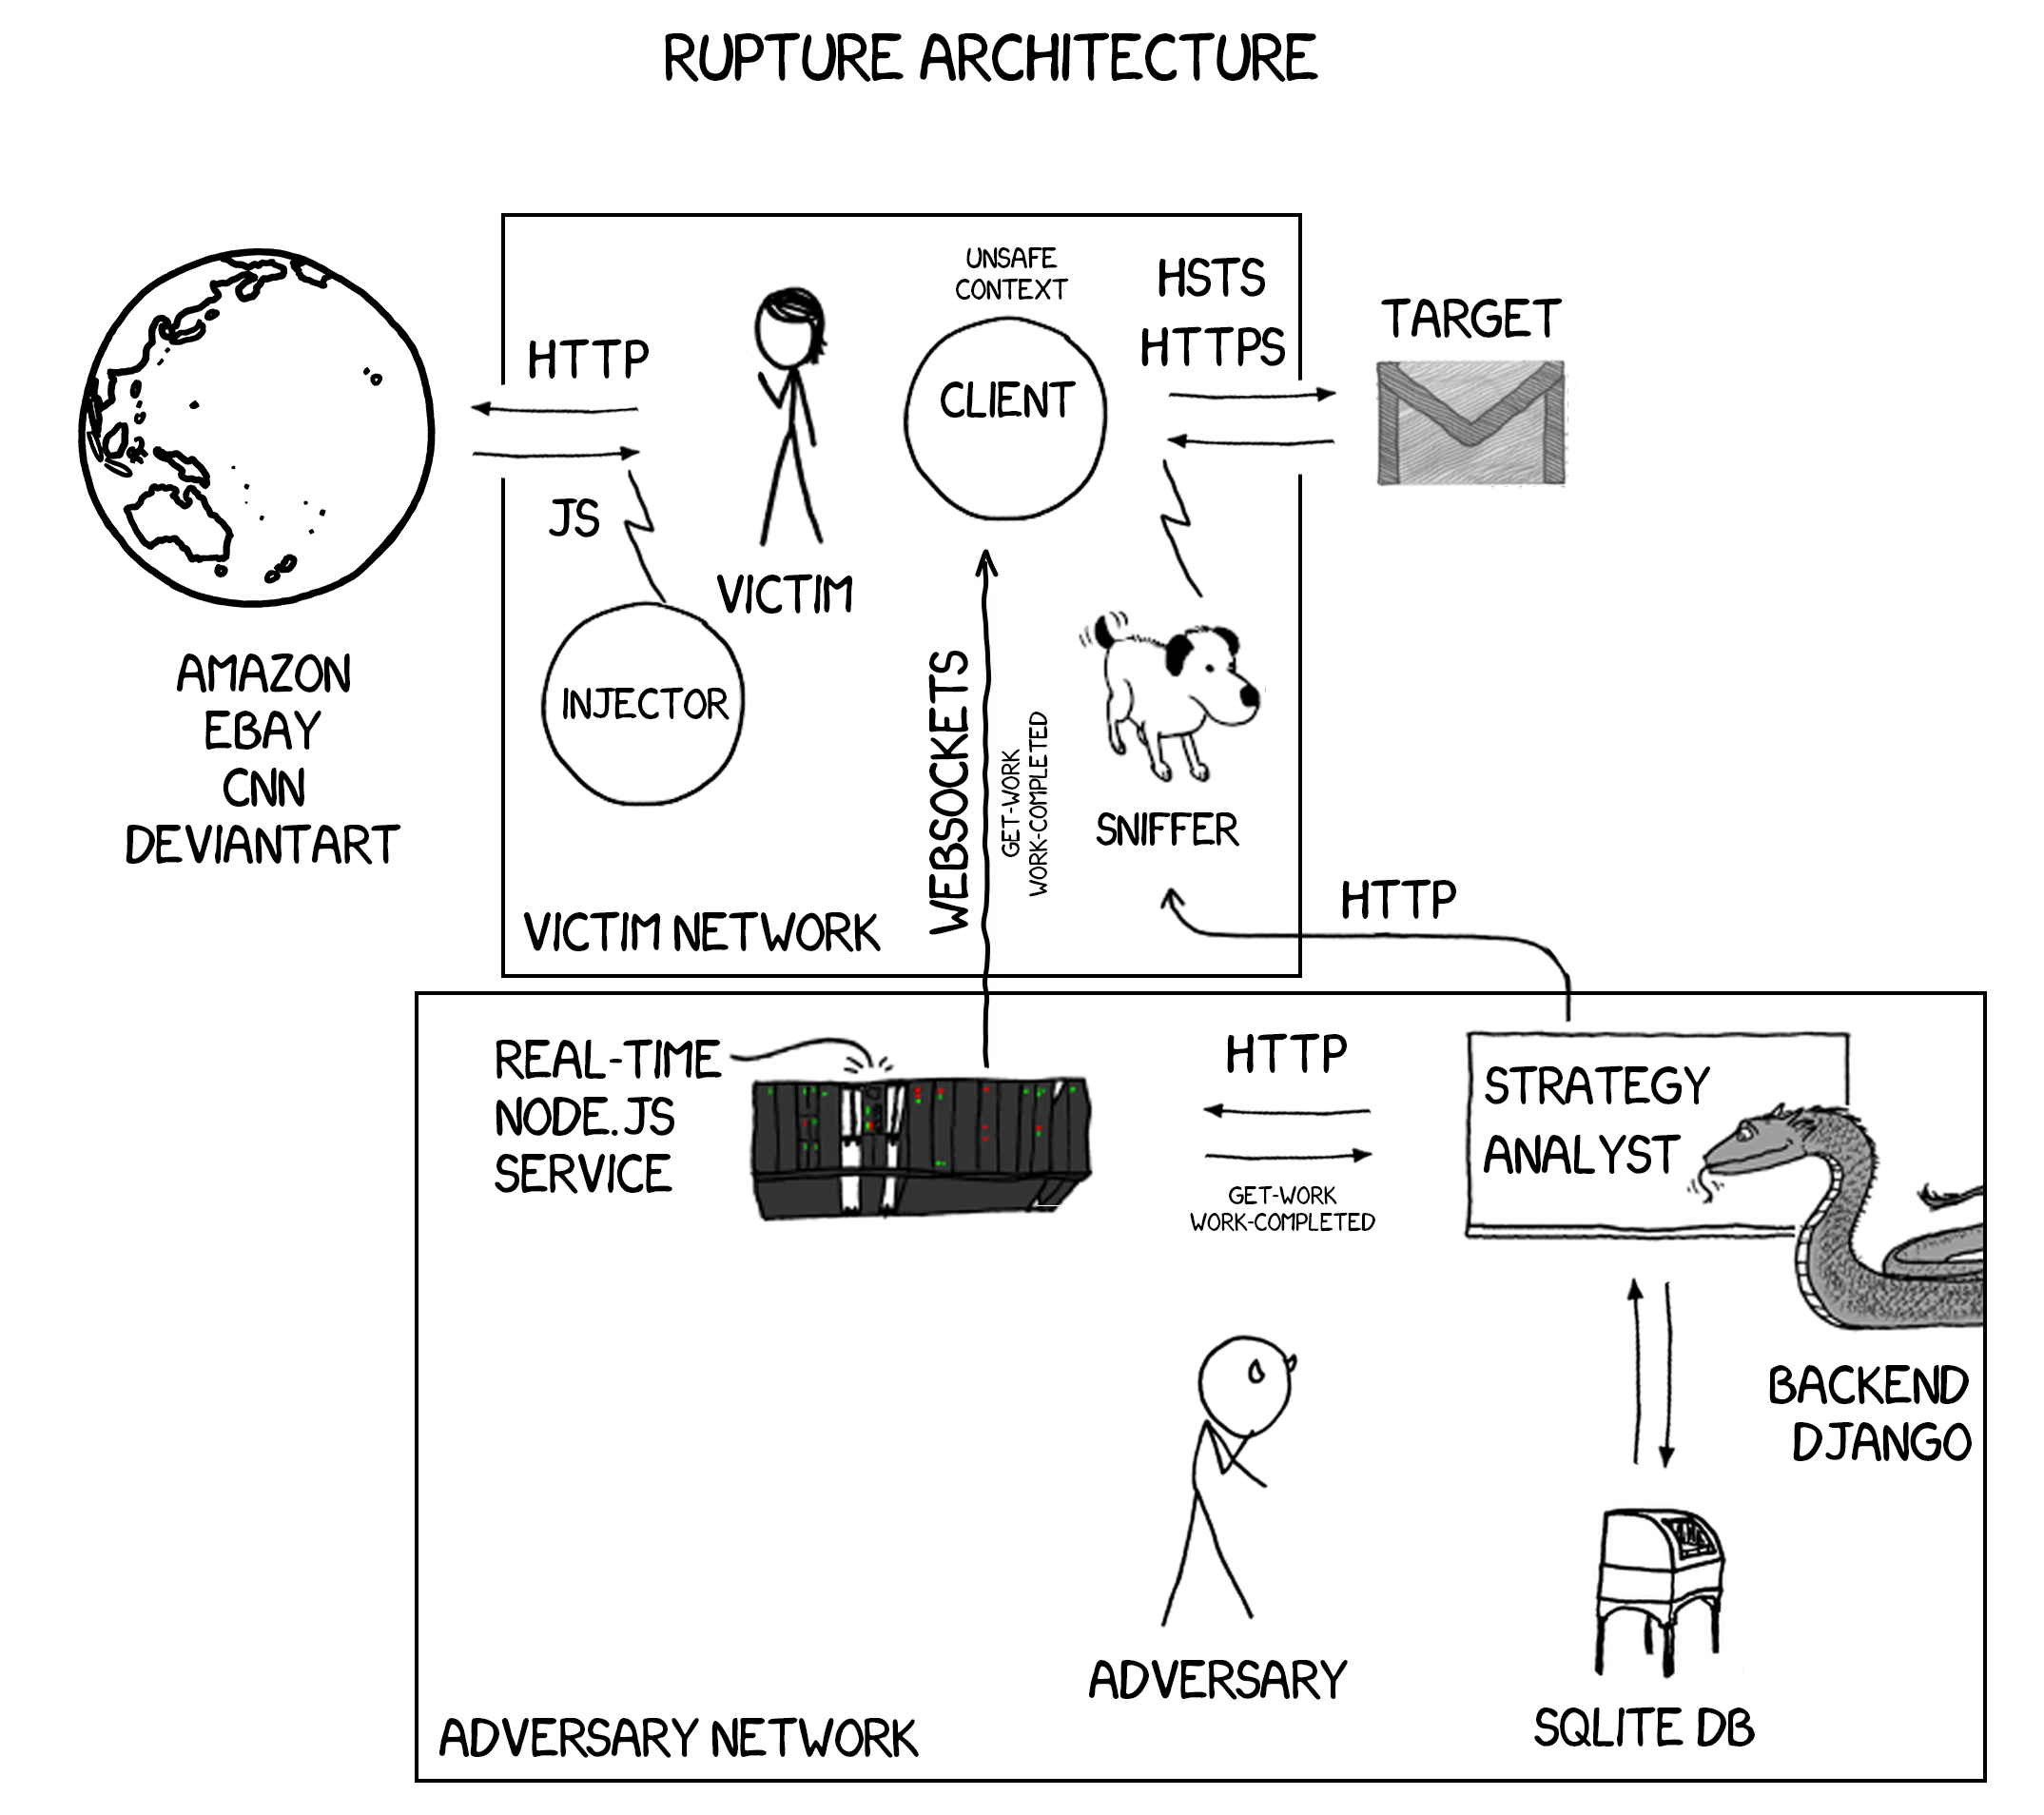
\includegraphics[width=120mm, height=95mm]{figures/architecture.png}
	\caption{Architecture}
	\label{fig:architecture}
\end{figure}

There are two underlying assumptions in our attack: The injection and the sniffing assumptions. These are often, but not necessarily, achieved through the same means.

\subsection{Injection}
The injection assumption states that the adversary is able to inject code that is run in the victim's browser. This may be achieved through various means, such as manipulating insecure HTTP responses from docking web services, different from the HTTPS target web service, on the victim’s network. Injection in Rupture is achieved through the injector component. We use bettercap~\cite{c10} to perform the HTTP injection. The injection is performed by ARP spoofing the local network and forwarding all traffic in a Man-in-the-Middle manner. It is simply a series of shell scripts that use the appropriate bettercap modules to perform the attack. The code that is injected is the client component. 

\subsection{Sniffing}
The sniffing assumption states that the adversary is able to observe network traffic between the victim and the target. This traffic is typically ciphertexts. Sniffing is achieved through the sniffer component. The sniffer component is responsible for collecting data directly from the victim's network. As the client issues chosen plaintext requests, the sniffer collects the respective ciphertext requests and ciphertext responses as they are sent on the network. These encrypted data are then collected and forwarded to the backend for further analysis and decryption. Our sniffer implementation runs on the same network as the victim, but it could in principle be operated at any node in the network path between the victim and the target. It is a Python program which uses scapy~\cite{c12} to collect network data.

\subsection{Client}
The client is responsible for issuing adaptive chosen plaintext requests to the target oracle. For this purpose, it receives commands through a command-and-control channel. These commands are sent to the client from the realtime component with which the client maintains a persistent connection.

\subsection{Realtime}
The realtime component is only responsible for communicating with the client. It can handle multiple targets and victims. It receives command-and-control connections from various clients which can live on different networks, orchestrates them, and tells them which ones will remain dormant and which ones will receive work, enabling one client per victim. The attack strategy is decided by the backend, which maintains a persistent attack state.

\subsection{Backend}
The backend is responsible for strategic decision taking, statistical analysis of samples collected, adaptively advancing the attack, and storing persistent data about the attacks in progress for future analysis.

At each stage of the attack, a prefix of the secret is known, because that portion of the secret has already been successfully decrypted. The known prefix grows until the whole secret becomes known, at which stage the attack is completed.

When a certain prefix of the secret is known, the next byte of the secret must be determined. The attack initially assumes the next unknown byte of the secret can come from the secret's alphabet, but slowly evaluates and rejects alphabet symbols until only one candidate symbol remains. At each stage of the attack of one byte of the secret, there is a certain known alphabet which the next byte can take. This known alphabet is a subset of the secret's alphabet.

To drill down on the known alphabet, one of two methods is employed. In the serial method, each symbol of the known alphabet is tried sequentially. In the divide \& conquer method, the alphabet is split into two candidate alphabet subsets which are tried independently. Additional methods are easy to implement. For example, a non-deterministic backtracking method could replace the deterministic serial or divide \& conquer methods. "Backtracking would choose characters which optimize a given utility function above a given threshold. All of these characters could then be added to a non-deterministic tree structure. The attack is able to choose among different methods, depending on the needs of the target.

The attack is conducted in rounds. In each round, a decision is made about the state of the attack and more information becomes known about the secret. In a round, either the next byte of the secret becomes known, or the known alphabet is drilled down to a smaller set. In order to compare various different candidate alphabets, the attack executes a series of batches of data collection for each round.

In each batch, several samples are collected for each candidate in the alphabet, forming a sampleset. A sample is the encrypted data pertaining to one response. When samplesets of the same amount of samples have been collected for all the candidates, a batch is completed and the data is analyzed. 

The analysis is performed by the analyzer which statistically compares the samples of different distributions and decides which distribution is optimal, i.e. contains the correct guess. This decision is made with some confidence, which is expressed in bytes. If the confidence is not strong enough, an additional batch of samplesets is collected, and the analysis is redone until the confidence value surpases a given threshold. The analyzer component is pluggable and can be replaced by different utility functions representing a different means of comparing probability distributions.

When enough batches have been collected for a decision to be made with good confidence, the round of the attack is completed and more information about the secret becomes known. Each round either decrypts one byte of the secret or reduces the candidate alphabet.

\section{RESTful API}

In this paper we implement for the first time a RESTful API via HTTP to which the user makes requests from the web User Interface. This RESTful API can also be used directly by programmers without the need to use the web interface.

\subsection{/victim}

The \textit{/victim} is an HTTP POST and GET endpoint. 

When the backend receives a POST request, it initiates a new attack. The arguments passed are the victim's IP and the target.  The backend creates and stores a new victim, creates the client and injection code for the specific victim and injects the client code to the victim's machine with bettercap. It returns HTTP 200 with a JSON that has a field "\textbf{victimid}", which contains the ID of the new victim.

On a GET request, the backend returns an HTTP 200 JSON response. The JSON contains a list of all the stored victims that the attack is still running on or has been completed.

\subsubsection{/victim/$ <victimId> $}

The /victim/$ <victimId> $ is an HTTP GET, PUT and DELETE endpoint.

On a GET request, the backend returns HTTP 200 with a JSON with details for the victim with the specific victimId. The argument passed is the victim's Id. The backend returns the general information and details of the attack. The general information consists of the victim's IP and machine name, the target name, the decrypted secret up to this point and a percentage of the progress. Further details are provided per  batch. These are the round number, the batch number, the alignment alphabet, the possible knownsecret and the confidence.

On a PUT request, the user asks the backend to pause or continue the attack. The argument passed is the desired state of the attack, either "paused" or "running". The backend updates the current state of the attack and returns HTTP 200.

On a DELETE request, the backend deletes the specific attack.

\subsubsection{/victim/notstarted}

The \textit{/victim/notstarted} is an HTTP GET endpoint. When a GET request is received, the backend scans the wifi network with bettercap to find all possible victims and their machine's name. The backend returns a list of possible's victims IPs and machine names.


\subsection{/target}
This is an HTTP 200 POST and GET endpoint.
On a POST request, the argument passed to the backend is the name of the target, the endpoint, the known prefix, the secret's alphabet, the secret length, the alignment alphabet, the records' cardinality and the method of the attack. The backend creates and stores the new target and returns 200 HTTP with a JSON with the target name.

On a GET request, the backend returns an HTTP 200 JSON response. The JSON contains a list of all the stored target for which an attack is possible.


\section{Web UI}

The user handles the attacks via a web interface which consists of two main pages and a modal window. The two main pages are the \textbf{Network Overview} and the \textbf{Victim Attack Inspection}. The modal window is used for the target configuration.

The Network Overview is the start page. It displays the completed, the currently running and the paused attacks. It also allows the user to initiate a new attack either by adding a custom victim or by scanning and choosing one of victims with bettercap (Figure~\ref{fig:start}).

\begin{figure}[thpb]
	\centering
	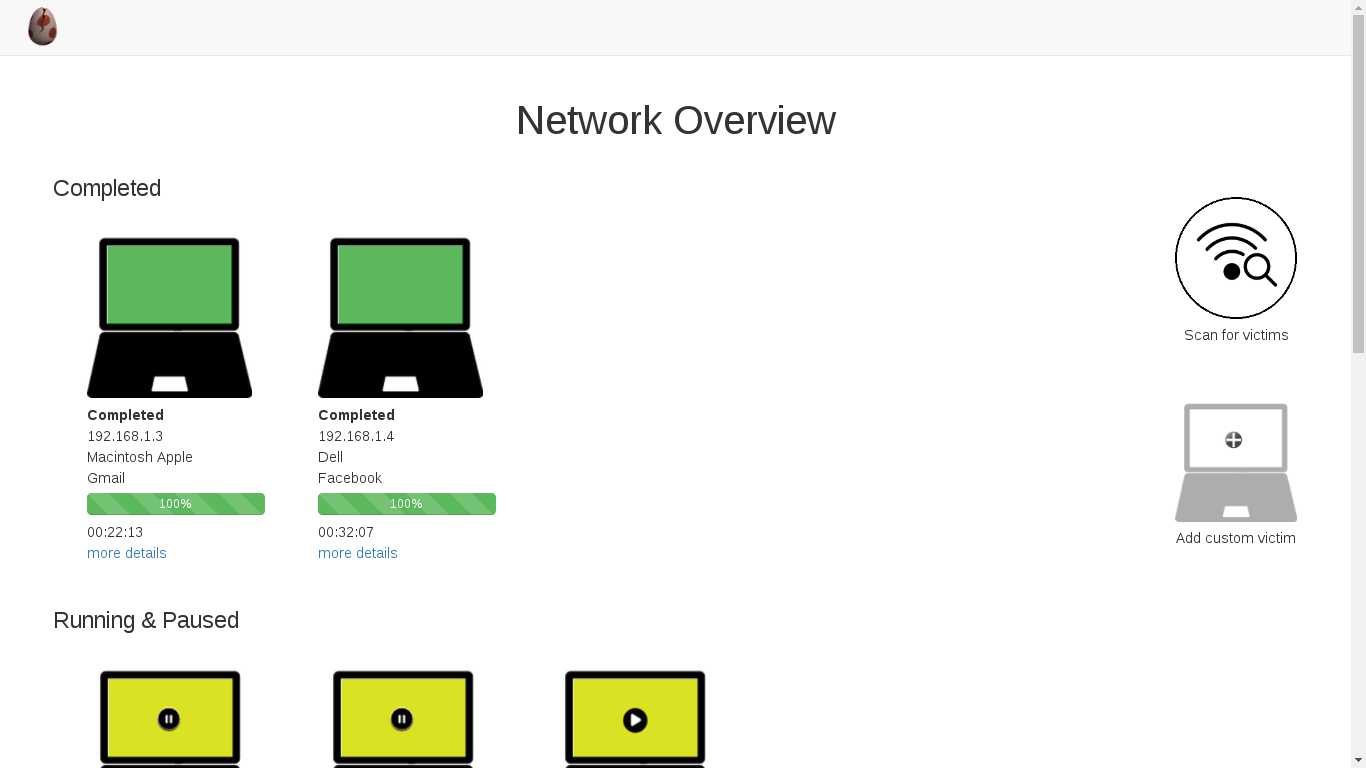
\includegraphics[width=100mm]{figures/startPage.png}
	\caption{Start Page}
	\label{fig:start}
\end{figure}

The completed and the running or paused attacks are represented PC icons. When the user clicks the \textit{Scan for victims} button, bettercap scans the network for possible victims, which are shown beneath the running/paused attacks (Figure~\ref{fig:attack}). The user can otherwise click \textit{Add custom victim} button if they already know the victim’s IP and don’t need to search for other victims.

\begin{figure}[thpb]
	\centering
	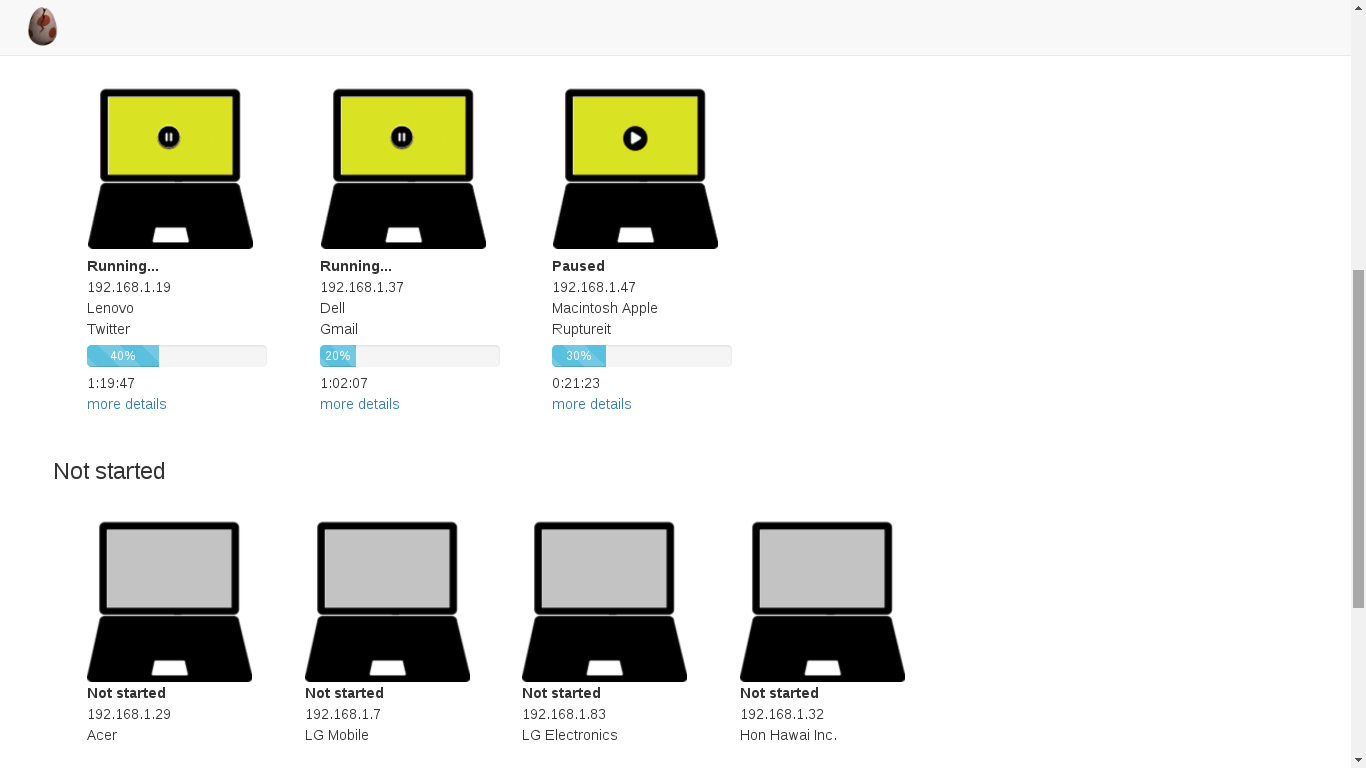
\includegraphics[width=95mm]{figures/notstarted.png}
	\caption{Possible victims for a new attack}
	 \label{fig:attack}

\end{figure}

The victim and target configuration are shown below. If the user has previously scanned the network, the victim's IP is already filled (Figure~\ref{fig:victim}).

\begin{figure}[thpb]
	\centering
	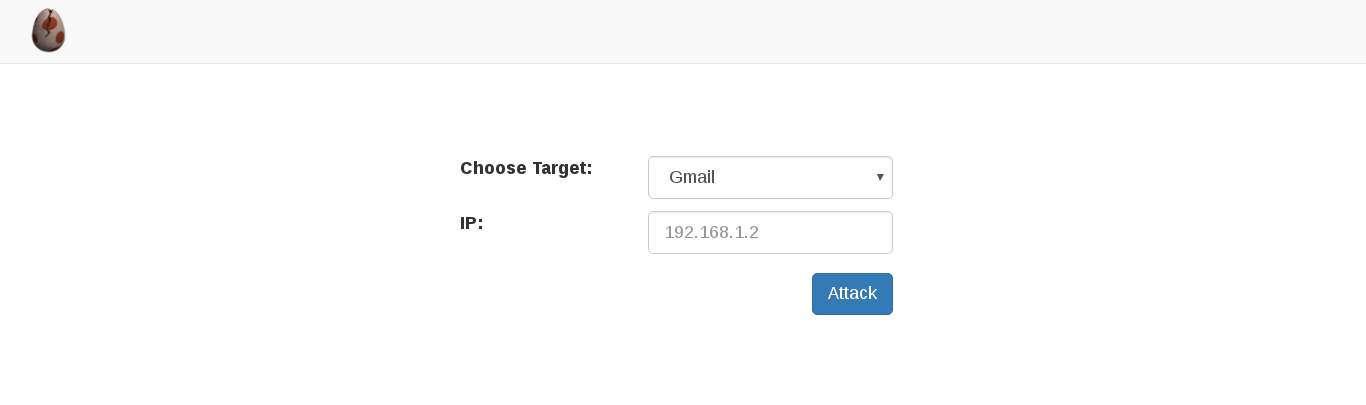
\includegraphics[width=95mm]{figures/victim.png}
	\caption{Victim Configuration}
	\label{fig:victim}
\end{figure}

There are some pre-configured targets but the user can configure a new one (Figure~\ref{fig:target}).


\begin{figure}[thpb]
	\centering
	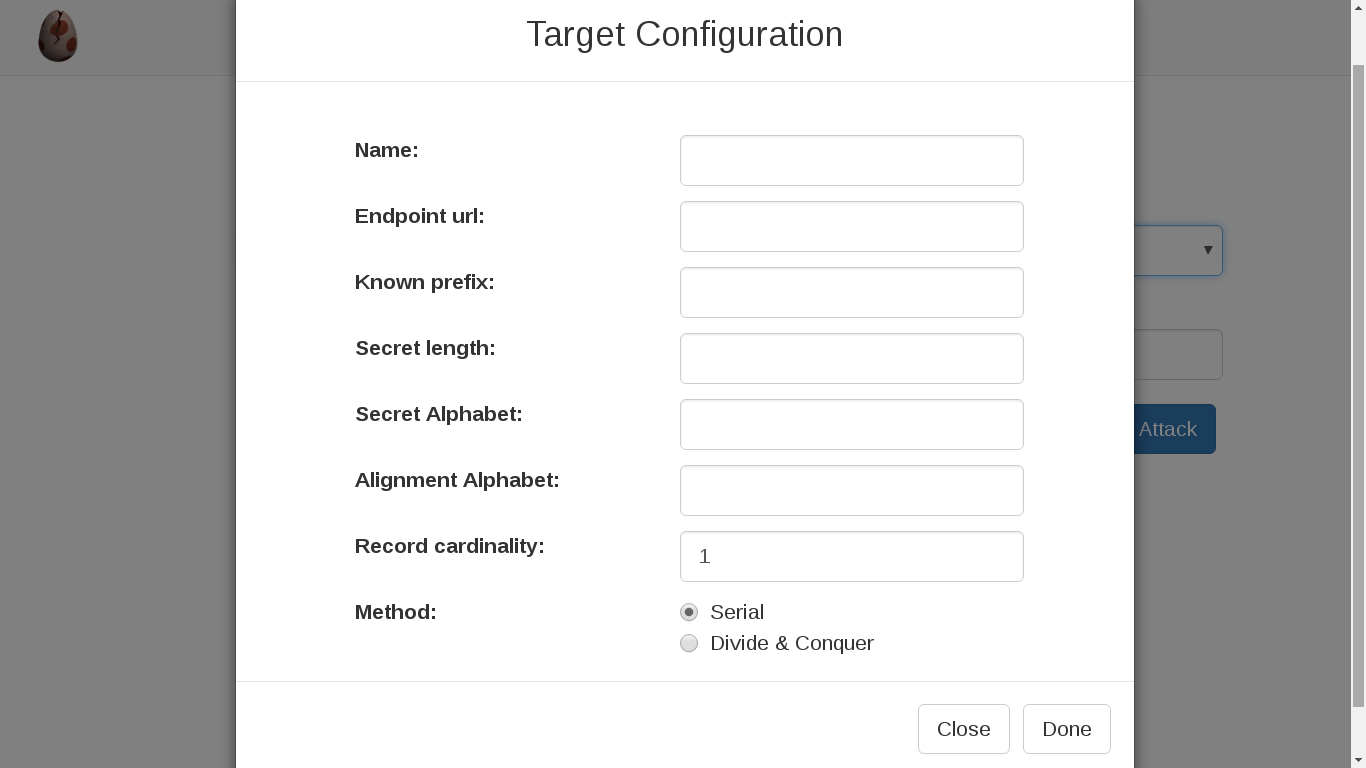
\includegraphics[width=90mm]{figures/target.png}
	\caption{Target Configuration}
	\label{fig:target}
\end{figure}

When the user clicks a completed, running or paused attack, they can view further details of the attack.

\begin{figure}[thpb]
	\centering
	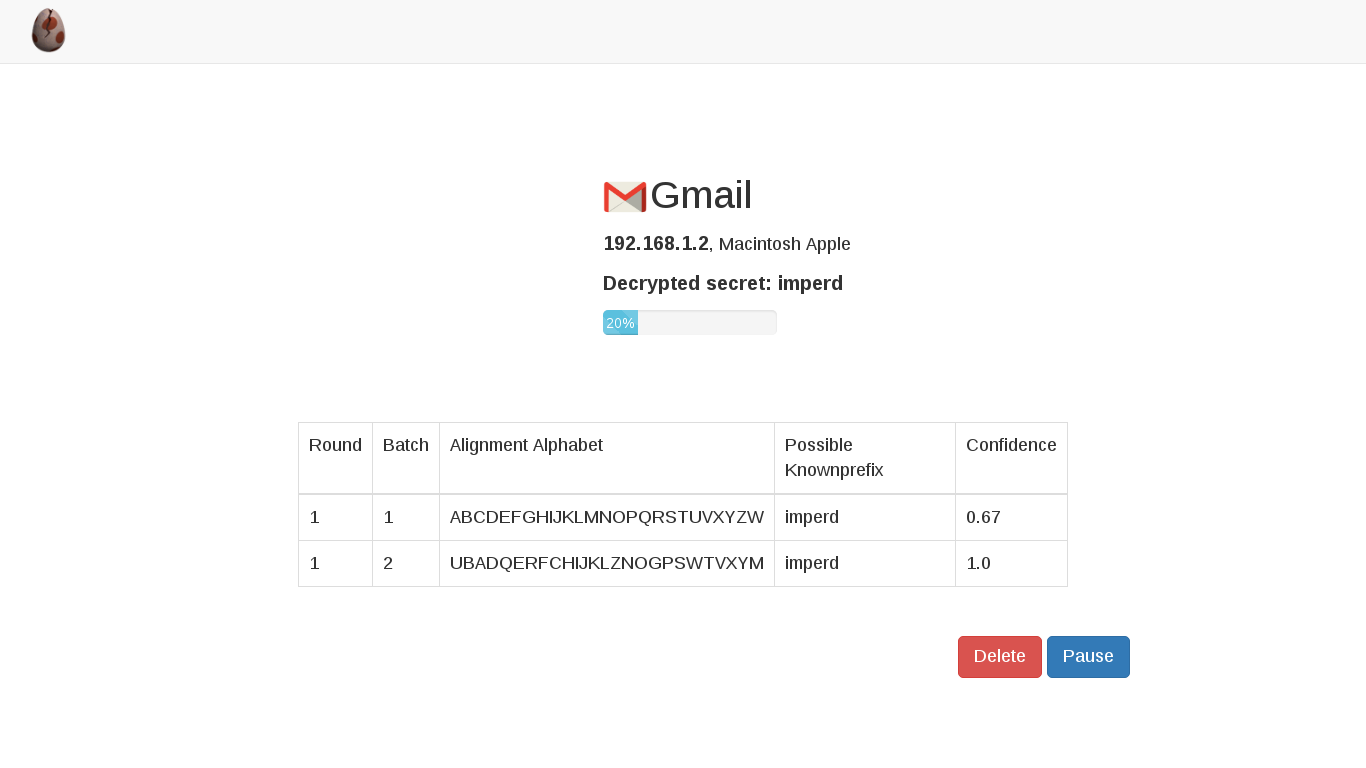
\includegraphics[width=115mm, height=75mm]{figures/attack.png}
	\caption{Attack details}
\end{figure}

The above indicate how easily the user can perform the attack in a fully automated way.

\section{Future work}

Rupture is a framework for conducting network attacks against web services and mostly focused on compression side-channel attacks.  Rupture provides a generalized scalable system for performing any attack on web services which requires a persistent command-and-control channel and attack adaptation and can be extended for CRIME,TIME~\cite{c18}, POODLE and HEIST.

Even the assumption that targets are HTTPS end-points can be relaxed. Any protocol that exchanges encrypted data on the network and for which a theoretical attack exists can in principle be attacked using Rupture. Examples of other encrypted protocols for which attacks can be tested include SMTP and XMPP.


\section{Related work}
Previous implementations of Rupture required scripting and a command line interface. The user had to edit the victim and target configuration scripts, run the attack setup and then initiate the attack. With the web interface, the initialization and initiation of the attack become automated. There is no need to manually scan the network with bettercap. All the user has to do is to configure the victim and target and press an $ Attack $ button. Also, the results are no longer presented as logs, but in a clear and readable way.

The browser exploitation framework (BeEF) hooks the victim's browser for an attacker to inject code, view cookies and browser history or even get a shell. Bettercap can also inject code, DNS spoof and manipulate HTTP/HTTPS or low level TCP traffic at runtime. Rupture uses some of these techniques in order to initiate the attack, but also analyzes the data and defines strategies for the next step.

\begin{thebibliography}{14}

\bibitem{c15}  D.Karakostas, D.Zindros: Practical New Developments in the BREACH Attack, Black Hat Asia, 2016

\bibitem{c17} J.Kelsey: Compression and information leakage of plaintext, FSE2002

\bibitem{c16} M. Vanhoef, Tom Van Goethem: HEIST: HTTP Encrypted Information can be
Stolen through TCP-windows, Black Hat USA 2016

\bibitem{c2} B. Moller, T. Duong, K. Kotowicz, This POODLE Bites: Exploiting the SSL 3.0 Fallback, September 2014.

\bibitem{c1} J. Rizzo, T. Duong: The CRIME attack, Ekoparty, 2012.

\bibitem{c3} Y. Gluck, N. Harris, A. Prado, BREACH: Reviving the CRIME attack,
Black Hat USA, 2013.

\bibitem{c14} D. Thai, J. Rizzo. "Here come the⊕ ninjas." Unpublished manuscript 320 (2011).

\bibitem{c18}T. Be'ery, A. Shulman: A Perfect CRIME? Only TIME Will Only TIME Will Tell, Black Hat Europe 2013

\bibitem{c10} [online] URL: \url{https://www.bettercap.org/} [cited March 2016]

\bibitem{c12} [online] URL: \url{http://www.secdev.org/projects/scapy/} [cited March 2016]

\bibitem{c19} [online] URL:https://github.com/dionyziz/rupture

\end{thebibliography}

\end{document}
